%%%%%%%%%%%%%%%%%%%%%%%%%%%%%%%%%%%%%%%%%
% The Szabo Book
% Structural Definitions File
% Version 0.1 (5/4/20)
%
% Author:
% dynamic_poker (dynamic_poker@outlook.com)
%
%
\RequirePackage{luatex85,shellesc}
\usepackage[top=1.39cm,bottom=1.8cm,left=1.7cm,right=1.27cm,headsep=10pt,papersize={13.8cm ,21.6cm}
]{geometry}
\usepackage{indentfirst} 
\usepackage{graphicx} % Required for including pictures
\graphicspath{{Pictures/}}
\usepackage{tikz,pgfplots} % Required for drawing custom shapes
%\pgfplotsset{compat=newest}
\usetikzlibrary{external}
\tikzexternalize[prefix=tikz/,
figure name=tikz_chap\thechapter_sec\thesubsection_no,
up to date check = md5,
]
\usepackage{booktabs,enumerate,threeparttable
} % Booktabs required for nicer horizontal rules in tables
\usepackage{xcolor} % Required for specifying colors by name
\definecolor{ocre}{RGB}{0,0,0} % Define the favorite color used for highlighting throughout the book
\bibliographystyle{alpha}


%-------------------------------------------------------------------
%	Chinese Settings
%-------------------------------------------------------------------
\usepackage[format=hang,labelfont=bf]{caption}
%\captionsetup{font={scriptsize}}
\captionsetup{figurename={图}, tablename={表}}
%\addto{\captionsenglish}{\renewcommand{\contentsname}{目\quad录}}
\def\chntoday{\the\year~年~\the\month~月~\the\day~日}
% adjust the width of tables to adapt it to the textwidth
\usepackage{tabularx}
\newcolumntype{Y}{>{\centering\arraybackslash}X} % New flag to centering the width-adapted columns

\usepackage{amsmath}
\usepackage{anyfontsize}
\usepackage{amssymb}
\usepackage{bm}

\usepackage{mathtools} % For *rcases* environment
\usepackage[scr=boondoxo, scrscaled=1]{mathalfa}
%\usepackage{mathrsfs}
\usepackage{mathptmx,mathpazo}
%\usepackage{old-arrows} % 
%\usepackage[T1]{fontenc}
%\usepackage{newpxtext,newpxmath}
%\usepackage{newtxtext}
%\usepackage{newtxmath,} %A systematic solution to Roman fonts, including math fonts.
\usepackage{braket,ulem}
\renewcommand{\braket}[1]{\Braket{#1}}
\renewcommand{\ket}[1]{\Ket{#1}}
\renewcommand{\bra}[1]{\Bra{#1}}
\usepackage[UTF8,scheme=plain]{ctex}
\usepackage{hyperref}
%\usepackage{fontspec}
%\usepackage{luatexja-fontspec}
%\setmainjfont{FandolSong}
%\setsansjfont{FandolKai}
\newcommand*{\refcs}[2]{
\hyperref[label]{text}
}

%-----------------------------------------------------------------
%	Page Headers
%-----------------------------------------------------------------

\usepackage{fancyhdr} % Required for header and footer configuration
\renewcommand{\chaptermark}[1]{\markboth{\sffamily\normalsize\chaptername\ \thechapter.\ #1}{}} % Chapter text font settings
\renewcommand{\sectionmark}[1]{\markright{\normalfont\normalsize\thesection\hspace{5pt}#1}{}}

%----------------------------------------------------------------------------------------
\let\bar\undifined
\newcommand{\bar}[1]{\overline{#1}}
\newcommand{\scr}[1]{\mathscr{#1}}
\newcommand{\bo}[1]{\mathbf{#1}}
\renewcommand{\epsilon}{\varepsilon}
\newcommand{\sch}{Schr\"odinger}
\newcommand{\ha}{Hamiltonian}
%\newcommand{\dd}{\text{d}}
\usepackage{xparse}
\newcommand{\dd}[1]{\mathrm{d}\mathbf{#1}}
\let\dd\undefined
\NewDocumentCommand{\dd}{ g }{%
	\IfValueTF{#1}
	{% https://tex.stackexchange.com/q/53068/5764
		\if\relax\detokenize{#1}\relax
		\mathrm{d} %
		\else
		\mathrm{d}\mathbf{#1}%
		\fi}
	{\mathrm{d}}%
}
\newcommand{\ddx}{\dd\mathbf{x}}

\newcommand{\db}[1]{\dd\bo{#1}}
\newcommand{\hs}{\mathscr{H}}
\newcommand{\vs}{\mathscr{V}}
\newcommand{\es}{\mathscr{E}}

\newcommand{\kaiti}{%\kaishu
}
\renewcommand{\emph}[1]{\textbf{#1}}


\usepackage{calc}
%use \settowidth, \widthof

\usepackage{endnotes}
\renewcommand{\makeenmark}{\hbox{$^\theenmark$}}
\renewcommand{\notesname}{\bf 注释}
\makeatletter
\@addtoreset{endnote}{chapter}
\makeatother
%\let\footnote\endnote

%-----------------------------------------------------------------
% the command to generate two lines between which are excerise content, using amsthm to number the exercise.
\let\openbox\undefined
\usepackage{amsthm}
\newtheoremstyle{nx}{}{}{\normalfont}{}{\bfseries}{}{1em}{}
\theoremstyle{nx}
\newtheorem{Xercise}{$\quad$练习}[chapter]
\newenvironment{xercise}{\par\vspace{\baselineskip}\noindent\hrule\vspace{.5\baselineskip}\Xercise}
{\vspace{\baselineskip}\hrule\par\endXercise}

\newcommand\Next{\endXercise\hrule\Xercise}
\newcommand{\exercise}[1]{\begin{xercise}#1\end{xercise}}
%========================================================

\newcommand{\tu}{\begin{figure}[h]
		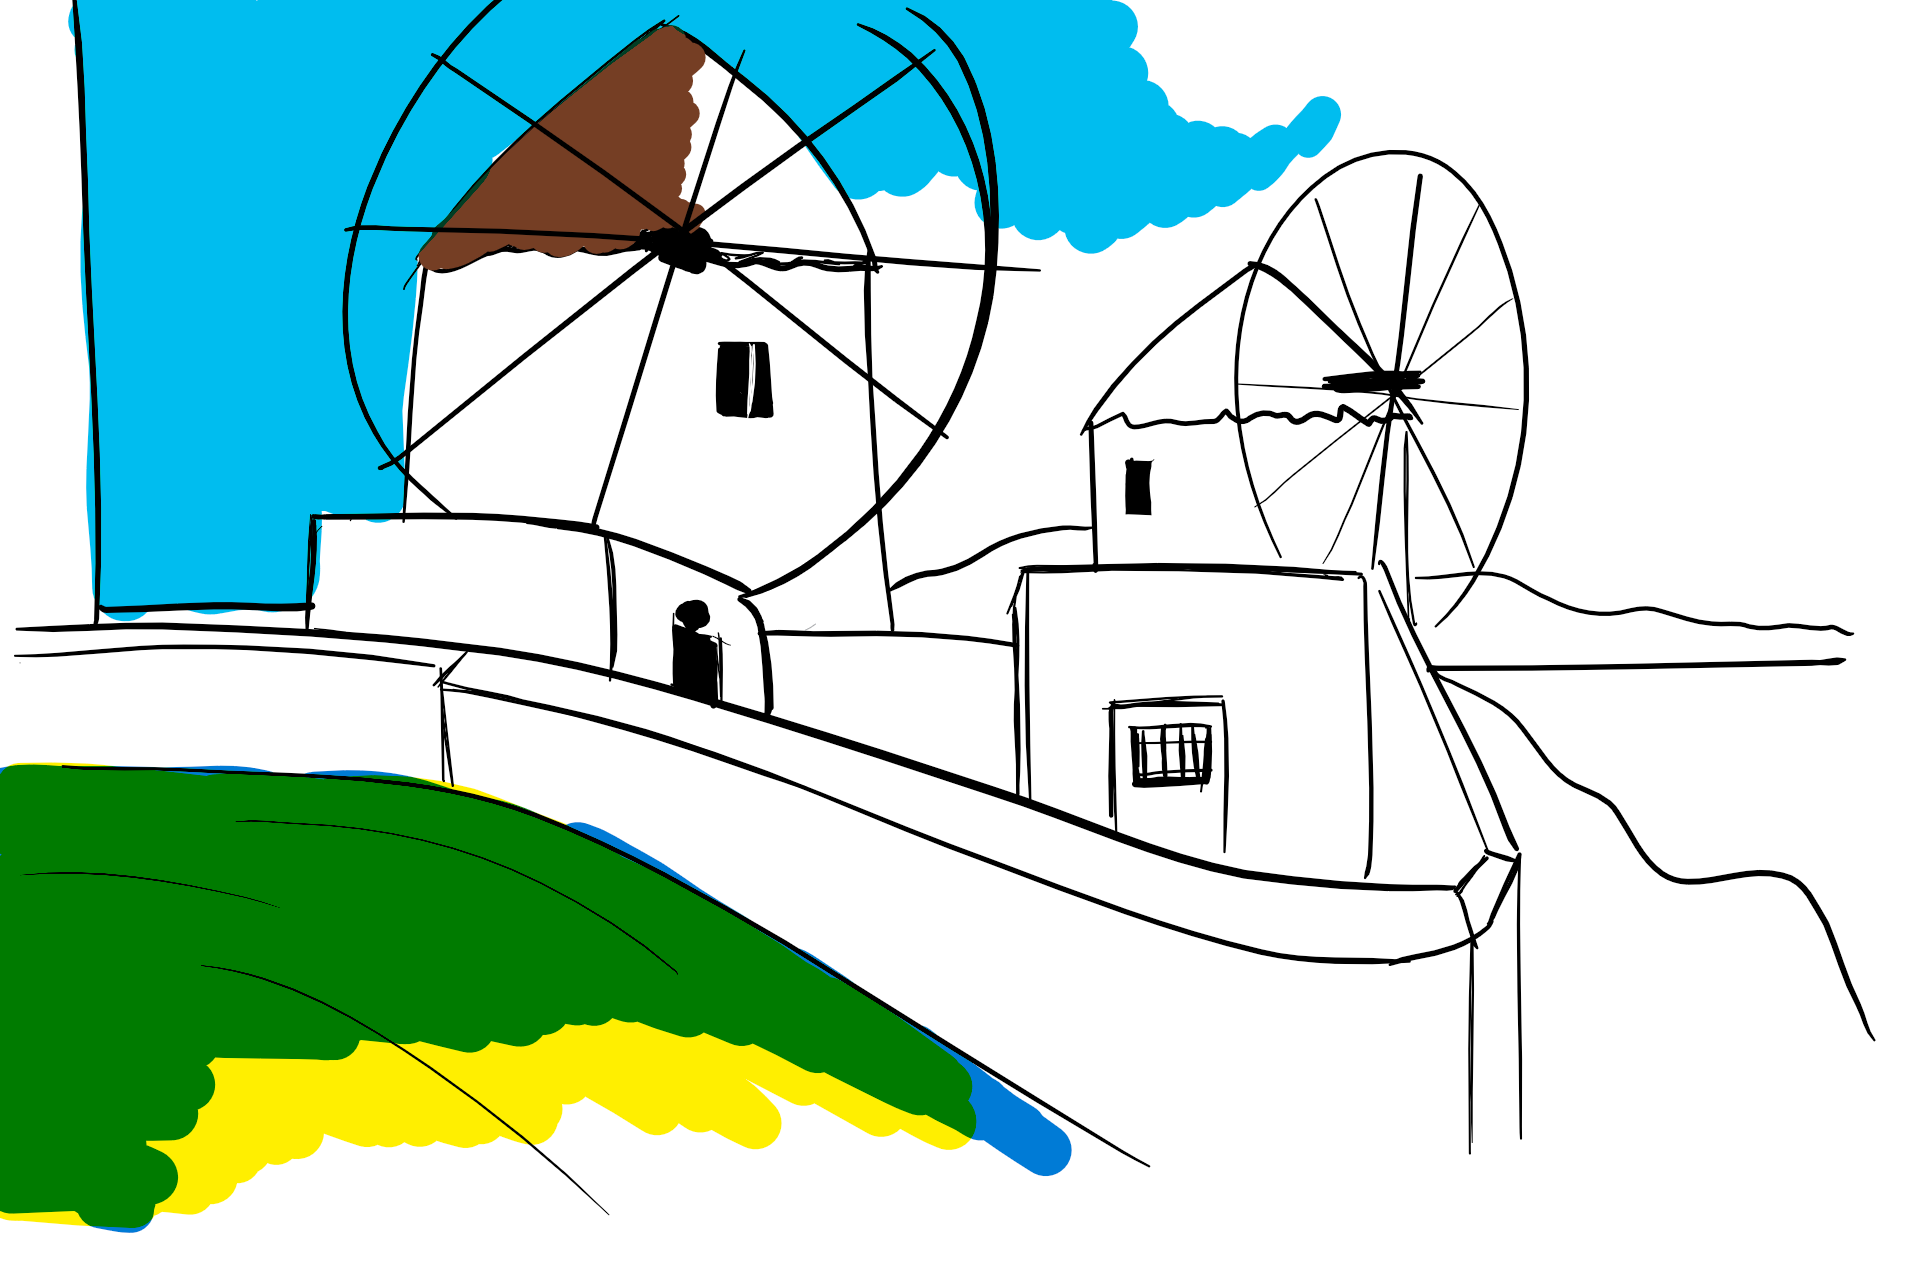
\includegraphics[width=.5\textwidth]{q.png}
\end{figure}}
% Feynman Diagram Setting
\usetikzlibrary{arrows.meta}
\newcommand{\midarrow}{\tikz \draw[-triangle 45] (0,0) -- +(.05,0);}
\tikzset{> = latex, color=blue}
\usetikzlibrary{decorations.markings,decorations.pathreplacing}
\tikzset{
	% style to apply some styles to each segment of a path
	on each segment/.style={draw=blue,
		decorate,
		    decoration={
			show path construction,
			moveto code={},
			lineto code={
				\path [#1]
				(\tikzinputsegmentfirst) -- (\tikzinputsegmentlast);
			},
			curveto code={
				\path [#1] (\tikzinputsegmentfirst)
				.. controls
				(\tikzinputsegmentsupporta) and (\tikzinputsegmentsupportb)
				..
				(\tikzinputsegmentlast);
			},
			closepath code={
				\path [#1]
				(\tikzinputsegmentfirst) -- (\tikzinputsegmentlast);
			},
		},
	},
	% style to add an arrow in the middle of a path
	mid arrow/.style={postaction={decorate,decoration={
				markings,
				mark=at position #1 with {\draw[arrows = {-Latex[width=0pt 7, length=5pt]}] (0pt,.0pt) -- (1.8pt,0pt);}
	}}},
	mid arrow/.default={.55},
	mid arrow seg/.style={postaction={on each segment={decorate,decoration={
				markings,
				mark=at position #1 with {\draw[arrows = {-Latex[width=0pt 7, length=5pt]}] (0pt,.0pt) -- (1.8pt,0pt);}}
	}}},
	mid arrow seg/.default={.55},
	% style to add an reverse arrow in the middle of a path
	mid reverse arrow/.style={postaction={decorate,decoration={
			markings,
			mark=at position .45 with {\draw[arrows = {-Latex[width=0pt 7, length=5pt]}] (1.8pt,.0pt) -- (0pt,0pt);}
	}}},
	mid reverse arrow seg/.style={postaction={on each segment={decorate,decoration={
				markings,
				mark=at position #1 with {\draw[arrows = {-Latex[width=0pt 7, length=5pt]}] (1.8pt,.0pt) -- (0pt,0pt);}}
	}}},
	above arrow/.style={to path={-- ++(0, .2) -| (\tikztotarget)},arrows = {-Latex[width=0pt 7, length=5pt]}},
	below arrow/.style={to path={-- ++(0,-.2) -| (\tikztotarget)}}
}
\newlength{\wletter}
\newlength{\hletter}
\newcommand{\tikzmark}[1]{
	\settowidth{\wletter}{\text{$\mathsurround=0pt i$}}
	\settoheight{\hletter}{\text{$\mathsurround=0pt i$}}
	\tikz[overlay,remember picture,inner sep=0,minimum height=\hletter] \node[shift={(-.4\wletter,.45\hletter)}] (#1) {};}
\newcommand{\dian}{\tikz{\filldraw[blue](0,0)circle(1pt);}}

\usetikzlibrary{calc}
%\usepackage[compat=1.1.0]{tikz-feynman}
\usepackage{float}
\renewcommand{\thefootnote}{\roman{footnote}} % Change the marks of footnotes to numbers
\usepackage{blkarray} %分块矩阵

%-----------------------------------------------------------------
%	Convinent abbreviations
%-----------------------------------------------------------------
\renewcommand{\normalsize}{\fontsize{8pt}{9.6pt}\selectfont}
\newcommand{\diagsize}{\fontsize{5pt}{6.6pt}\selectfont}
\newcommand{\cs}{a^\dagger}
\newcommand{\hd}{\mathrm{H}_2}
\newcommand{\hft}{Hartree-Fock}
\newcommand{\twoe}{r_{12}^{-1}}
\newcommand{\tp}{\tilde{\Phi}}
%\usepackage[symbol]{footmisc} 
\newcommand{\bfr}{\mathbf{r}}
\newcommand{\heh}{\mathrm{HeH}^+}
\newcommand{\au}{\,\mathrm{a.u.}}
\newcommand{\ts}{\mathscr{S}} %总自旋算符
\usepackage{xeCJKfntef} % the package containing the command \CJKuderline*{} for the \mci command
\newcommand{\mci}[1]{\CJKunderline*{#1}}
\newcommand{\phrase}[1]{\CJKunderline*{#1}}
%%为方便而定义的简单代替, 最后要全部换回来.
\newcommand{\jt}{\ket{\Phi_0}}
\newcommand{\hjt}{\ket{\Psi_0}}
\newcommand{\jtn}{\Phi_0}
\newcommand{\hjtn}{\Psi_0}

\usepackage{wasysym}
%For the symbol \CheckedBox
\usepackage{stackengine,scalerel}
\newcommand\DSquare{\ThisStyle{\ensurestackMath{%
            \stackinset{c}{}{c}{}{\scalebox{.5}{$\SavedStyle\blacksquare$}}
            {\SavedStyle\square}}}}
%For a filled box.
%CR: https://tex.stackexchange.com/questions/553834/is-there-a-intermediate-checkedbox-symbol-in-latex